\documentclass[a4paper, 12pt]{article}
\usepackage[utf8]{inputenc}
\usepackage[czech]{babel}
\usepackage[left=2cm, top=3cm, text={17cm, 24cm}]{geometry}
\usepackage{graphicx}
\usepackage{fancyhdr}
\usepackage{enumitem}
\usepackage[T1]{fontenc}
\usepackage{tikz}
\usepackage{tikz-qtree}
\usetikzlibrary{shapes.geometric}
\usetikzlibrary{calc,shapes.multipart,chains,arrows}
\makeatletter
\newcommand*{\rom}[1]{\expandafter\@slowromancap\romannumeral #1@}
\makeatother
\usepackage[unicode]{hyperref}
\hypersetup{
	colorlinks = true,
	hypertexnames = true,
	citecolor = red
}

\setlength{\headheight}{15pt}

\begin{document}

    %Titulni strana
    \begin{titlepage}
        \begin{center}
            
\includegraphics[width=0.87\textwidth]{images/logo_cz.png}
            \vspace*{6cm}

            \Huge{\textbf{Dokumentace}}
            \vspace{0.5cm}
            
            \LARGE{Implementace překladače imperativního jazyka IFJ24}
            \vspace{0.5cm}
            
            \Large{Tým xbohatd00, Varianta - TRP-izp}
            \vspace{2.5cm}
            
            \large{\textbf{Daniel Bohata} (xbohatd00) 25\%}
            \vspace{0.1cm}
            
            \large{Tadeáš Horák (xhorakt00) 25\%}
            \vspace{0.1cm}
            
            \large{Ivo Puchnar (xpuchn02) 25\%}
            \vspace{0.1cm}
            
            \large{Adam Vožda (xvozdaa00) 25\%}
            \vspace{0.1cm}
            
           \vfill
		   \begin{flushleft} 
		   \large
		   Rozšíření: FUNEXP
		   \hfill
		   Brno, \today
		   \end{flushleft}
        \end{center}
    \end{titlepage}

\pagestyle{fancy}
\lhead{\bfseries Překladač IFJ24}
\rhead{\bfseries Obsah}

\newpage
\tableofcontents

%%%%%%%%%%%%%%%%%%%%%%%%%%%%%%%%%%%%%%%%%%%%%%%%%%%%%%%%%%%%%%%%%%%%%%%%%%%%%%%%%
\newpage
\rhead{\bfseries Práce v týmu}
\section{Práce v týmu}
\subsection{Rozdělení práce mezi jednotlivé členy týmu}
\begin{itemize}
    \begin{minipage}{0.5\linewidth}   
        \item Daniel Bohata
        \begin{itemize}
        \item[-] Vedení
        \item[-] Návrh ASS
        \item[-] Generace kódu 
        \end{itemize}
        \item Tadeáš Horák
        \begin{itemize}
        \item[-] Návrh ASS
        \item[-] Implementace ASS
        \item[-] Sémantická analýza
        \end{itemize}
        \item Ivo Puchnar
        \begin{itemize}
        \item[-] Lexikální analýza
        \item[-] Dokumentace
        \end{itemize}
        \item Adam Vožda
        \begin{itemize}
        \item[-] Implementace ASS
        \item[-] Syntaktická analýza
        \end{itemize}
    \end{minipage}
\end{itemize}

\newpage
\subsection{Průběh práce}
Na projektu jsme začali pracovat hned. Po značném rozpracování tabulky symbolů, lexikální a syntaktické analýzy jsme ale práci pozastavili. K projektu jsme se naplno vrátili během 8. týdne po půlsemestrálních zkouškách. Následně se naše úsilí zvyšovalo s blížícím se termínem. Každý si vzal určitou část s tím, že jsme si navzájem pomáhali, když někdo potřeboval. Vedoucí nenechával nic náhodě, ale nevytvářel přílišný nátlak.
\subsection{Sdílení kódu}
Pro sdílení kódu jsme použili Git/GitHub. Systém za nás udržoval přehled o verzích a jejich kompatibilitě. Pro každou část jsme vytvořili zvláštní větev. Po dokončení části jsme větev spojili s větví \textit{main}, kde jsme udržovali plně funkční program.
\subsection{Komunikace}
Seznámení týmu proběhlo osobně. Následná komunikace probíhala hlavně přes skupinové zprávy na Instagramu. Když bylo potřeba sdílet nějaký soubor nebo více obrázků, použili jsme skupinu na Discordu. Prezentaci na obhajobu jsme rovněž udělali na osobní schůzce.

%%%%%%%%%%%%%%%%%%%%%%%%%%%%%%%%%%%%%%%%%%%%%%%%%%%%%%%%%%%%%%%%%%%%%%%%%%%%%
\newpage
\rhead{\bfseries Implementace překladače (Lexikální analýza)}
\section{Lexikální analýza}
Lexikální analýza se provádí funkcí \textit{get\_token()}, která je definována v souboru \textit{Lexem\_an.c}. Její pomocné struktury a funkce jsou definovány v souborech \textit{tokens.h, .c}.\newline
Syntaktická analýza zavolá \textit{get\_token()}, který vrací strukturu \textit{Token}. Druh tokenu se určuje podle atributu \textit{KeyWord kw}. V atributech \textit{int i, double f, char *s} se předávají hodnoty tokenů pro identifikátory, čísla a stringy.\newline
Lexikální analyzátor jsem vytvořil z lexikálních analyzátorů, které jsem udělal pro projekty posledních dvou let.

\subsection{Inicializace}
Na začátku se zavedou proměnné a alokuje paměť.\newline
Proměnné \textit{int n} a \textit{double d} slouží k předání celých a desetinných čísel do tokenů. \textit{Token new} drží strukturu \textit{Token}, kterou funkce po úpravách lexikální analýzou vrací. \textit{char letter} si pamatuje poslední znak ze vstupu. Pokud funkce končí a poslední znak se nevyužil, vrací ho zpět na vstup. \textit{size\_t lex\_size} udržuje aktuální maximální alokovanou délku \textit{char *lexem}. Při spuštění funkce začíná na 8. \textit{char *lexem} je dynamicky alokovaný string pro uchovávání dlouhých lexémů. Před přidáním dalšího znaku funkce zkontroluje, zda má \textit{*lexem} dostatek místa. Pokud ne, realokuje jeho obsah s dvojnásobnou velikostí a tu zapíše do \textit{lex\_size}. \textit{char *p} je pomocný pointer. Při realokaci \textit{*lexem} na něm zjistíme, zda realokace proběhla úspěšně, a při předávání stringu do tokenu do něj alokujeme adekvátní velikost stringu. Alokovanou paměť následně předáme do atributu \textit{*s} tokenu.

\subsection{Postupná úprava analyzátoru}
První verze lexikálního analyzátoru fungovala tak, že se funkce zavolala zvlášť před ostatními analýzami a vytvořila jednostranně vázaný, který pak mohli procházet, ale pro splnění podmínky syntaxí řízené analýzy jsme ho změnili na vracení jednotlivých tokenů. V kódu můžete najít některé pozůstatky této verze, např. while cyklus pod inicializací. Pokud prvek neubíral funkčnosti, ponechali jsme ho.

\subsection{Určování tokenu}
Funkce \textit{get\_token()} rozhoduje o tokenu podle příchozího znaku. Tento znak vloží do velkého switche.\newline
Na začátku switche najdeme bílé znaky, které analyzátor přeskočí. Komentáře se rovněž přeskakují, jen se nacházejí níže.\newline
Následují jednoznačné tokeny. Jinak řečeno, tokeny vyžadující pouze 1-2 znaky.\newline
Víceřádkové stringy se poznají podle dvou obrácených po sobě jdoucích lomítek "\textbackslash\textbackslash" a posílají se stejně jako řádkové, v atributu tokenu \textit{*s} s atributem \textit{kw} nastaveným na \textit{text}. Rozdíl je v jejich tvorbě. Do stringu se přidá vše, co se nachází za "\textbackslash\textbackslash", včetně konce řádku '\textbackslash n'. Samotná lomítka se neposílají. Pokud se na dalším řádku, po bílých znacích, nachází další "\textbackslash\textbackslash", proces se opakuje, jinak se poslední '\textbackslash n' smaže a token se pošle.\newline
Jednořádkové stringy se poznají podle dvojitých uvozovek ". Pokud následují dvě " po sobě, jedná se o prázdný string a může se tedy ihned poslat token s \textit{text}. V \textit{*s} se pošle pouze '\textbackslash0'. Pokud následují znaky, přidají se do odevzdávaného stringu. Pokud cyklus narazí na obrácené lomítko '\textbackslash' vyzkouší, zda se jedná o escape sekvenci. Pokud ne, dojde k chybě 1. Pokud následuje 'x', zkontroluje se, zda následující dva znaky odpovídají zápisu hexadecimálního čísla. Pokud ano, hodnota se převede na znak, který se přidá do stringu, jinak nastává chyba 1. Druhé " ukončí nabírání znaků a pošle se token. String se posílá bez ohraničujících ".\newline
Mezi celými a desetinnými čísly rozlišujeme podle přítomnosti tečky nebo exponentu. Čísla začínají jako celá po příchodu číslovky, tedy znak 0 až 9. Pokud jako první přijde 0 a následují další číslice, jedná se o chybu 1. Pokud po číslovkách následuje '.' nebo 'e' číslo je jednoznačně desetinné. Po '.' a alespoň jedné číslovce může stále přijít 'e'. Po 'e' musí také následovat alespoň jedna číslovka. Před ní se může objevit '+' nebo '-'. Pokud přijatý znak už není jeden z jmenovaných, string se převede na číslo, vloží se do atributu \textit{i} pro celá a \textit{f} pro desetinná čísla. Pro jistotu se číslo pošle i jako string v \textit{*s}.\newline
Identifikátory a klíčová slova začínají buď písmeny nebo podtržítkem '\_'. Pokud za '\_' nenásledují písmena, čísla ani '\_', jedná se o prázdnou proměnnou a odevzdá se její token. V opačném případě se do řetězce pomocí cyklu vezmou všechny zmíněné znaky. Aby se snížila režie, porovná se první znak řetězce s prvními znaky všech možných klíčových slov. Tam, kde se shodují, se řetězec porovná s konkrétním klíčovým slovem, díky čemuž se vynechají porovnávání s ostatními. Pokud se řetězec shoduje s celým slovem, vyšle se jeho token, jinak se vyšle token \textit{id}, s řetězcem v \textit{*s}.\newline
Pokud funkce najde EOF, pošle token \textit{end} pro oznámení konce souboru.\newline

\subsection{Vysvětlení konečného automatu}
\begin{itemize}
    \item Ovály s jednoduchým okrajem jsou obyčejné stavy a ovály s dvojitým okrajem jsou stavy konečné.
    \item Pro přehlednost jsou některé přechody mezi stavy spojeny do jedné čáry. Pokud tomu tak je, symbol, který přechodu náleží, je vyobrazen tak, aby se nedaly zaměnit. Buď u jednotlivých přechodů, nebo u přechodů se stejným znakem směřujících do stejného stavu. 
    \item Některé přechody mají šipku oběma směry. To znamená, že se při správném znaku lze vrátit do předchozího stavu.
    \item U hledání identifikátorů automat zůstává ve stavu \textit{id}, dokud řetězec neodpovídá celému klíčovému slovu. Poté přejde do odpovídajícího stavu. Pokud ale řetězec pokračuje vrací se do \textit{id}, kde už zůstává.
    \item Pokud automat dojde do konečného stavu a dostane znak neodpovídající žádnému z jeho přechodů, znak vrátí na vstup a odešle token odpovídající aktuálnímu konečnému stavu s případným obsahem (číslo/string).
    \item Pokud automat dojde do běžného stavu a dostane znak neodpovídající žádnému z jeho přechodů, dochází k chybě číslo 1, chyba v lexému, a program končí.
    \item Automat začíná velkým stavem \textit{start} vlevo uprostřed. Vlevo nahoře se nachází oblast tokenů tvořených 1-2 znaky. Vpravo nahoře jsou klíčová slova a identifikároty proměnných a funkcí. Vpravo uprostřed jsou víceřádkové stringy. Vpravo dole jsou jednořádkové stringy
\end{itemize}

\newpage
\subsection{Diagram konečného automatu}
\begin{figure}[ht!]
    \begin{center}
        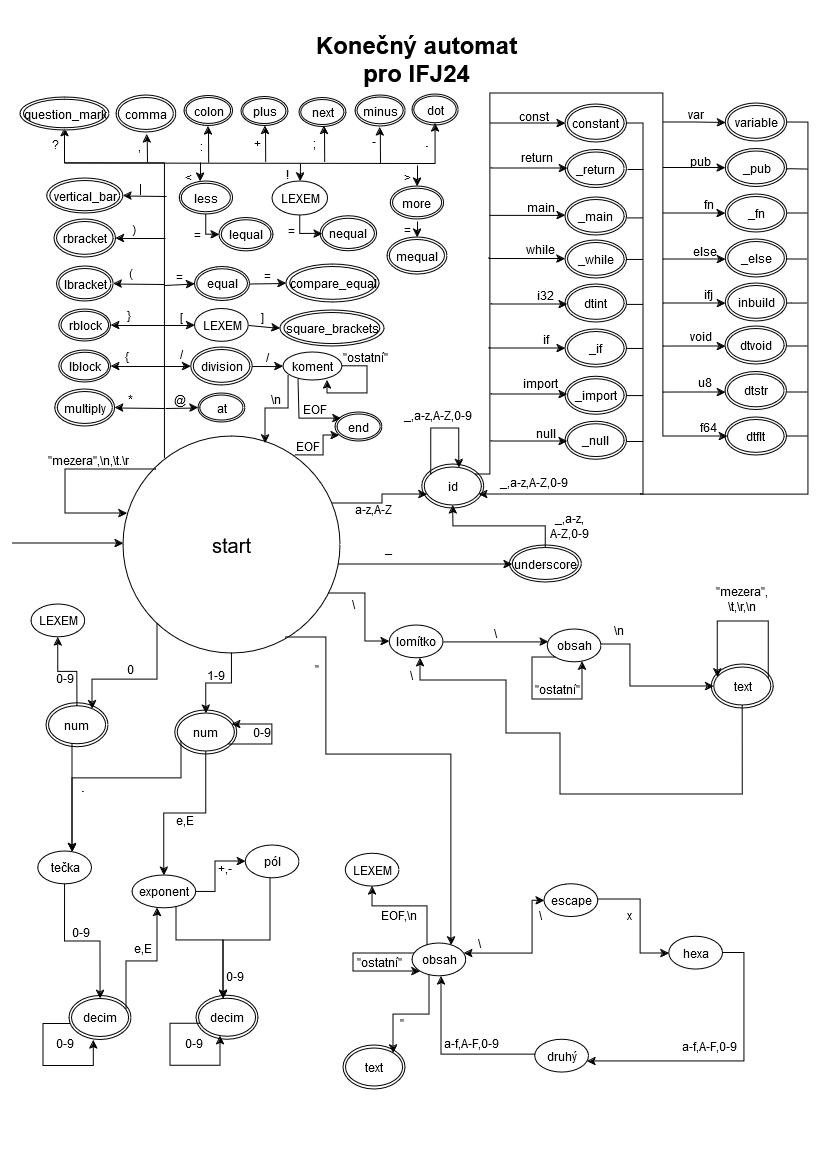
\includegraphics[origin=c, width=0.8\textwidth]{images/FSM_IFJ24.drawio.png}
        \caption{Diagram konečného automatu}
    \end{center}
\end{figure}

%%%%%%%%%%%%%%%%%%%%%%%%%%%%%%%%%%%%%%%%%%%%%%%%%%%%%%%%%%%%%%%%%%%%%%%%%%%%%%%%
\newpage
\rhead{\bfseries Implementace překladače (Syntaktická analýza)}
\section{Syntaktická analýza}

Syntaktická analýza je implementována v souboru \texttt{syntax\_an.c} (s odpovídajícím hlavičkovým souborem \texttt{syntax\_an.h}) a je realizována pomocí rekurzivního sestupu na základě LL gramatiky. Tento soubor obsahuje klíčovou funkci překladače, \textit{syntax\_analyzer()}, která provádí veškeré potřebné operace před a po syntaktické analýze.

Proces začíná voláním funkce \textit{headers()}, která načte počáteční pravidlo (import) a následně zpracovává hlavičky funkcí. Tyto hlavičky jsou uloženy do symbolické tabulky, zatímco těla funkcí jsou během prvního průchodu ignorována. Po načtení hlaviček se vstupní proud resetuje na začátek souboru pomocí funkce \textit{rewind\_stdin()}.

Následuje druhý průchod, zahájený voláním funkce \textit{program()}, který provádí podrobnou analýzu celého programu. V tomto kroku se také provádí sémantická kontrola a vytváří se abstraktní syntaktický strom (AST). AST je generován pomocí funkcí, které vytvářejí jednotlivé uzly a propojují je do hierarchické struktury. Po dokončení syntaktické analýzy je AST předán do fáze generace kódu.

Tokeny jsou načítány lexikálním analyzátorem prostřednictvím funkce \textit{read\_token()}, která volá funkci \textit{get\_token()}. Tato funkce slouží jako rozhraní mezi lexikální a syntaktickou analýzou. Parser zpracovává všechny části LL gramatiky s výjimkou výrazů. Výrazy jsou předávány metodě precedenční syntaktické analýzy, která je samostatně vyhodnocuje.

\subsection{Přechod mezi rekurzivním sestupem a precedenční analýzou}
Přechod mezi rekurzivním sestupem a precedenční analýzou je realizován voláním funkce \textit{expressionParser(bool tokenRead, ast\_node\_exp\_t **resultPointer)} ve souboru \texttt{expression\_parser.c}. Tato funkce je volána na místech, kde se očekává výraz, například za symbolem \texttt{=}. Parametr \texttt{tokenRead} indikuje, zda byl první token již přečten, a parametr \texttt{resultPointer} slouží jako ukazatel, kam je uložen výsledný strom výrazu.

\vspace{4cm}

\newpage

\subsection{LL gramatika}

\begin{enumerate}
    \item Program → Import Function\_list
    \item Import → \texttt{const} \texttt{ifj} \texttt{equal} \texttt{at} \texttt{lbrace} \texttt{text} \texttt{rbrace} \texttt{semicolon}
    \item Function\_list → Function\_analysis Function\_next
    \item Function\_next → \texttt{end}
    \item Function\_next → Function\_list
    \item Function\_analysis → \texttt{pub} \texttt{fn} \texttt{id} \texttt{lbrace} Param\_def \texttt{rbrace} Return\_type \texttt{lblock} Code\_list \texttt{rblock}
    \item Param\_def → eps
    \item Param\_def → Param Param\_list
    \item Param\_list → \texttt{comma} Param\_def
    \item Param\_list → eps
    \item Param → \texttt{id} \texttt{colon} Var\_type
    \item Return\_type → Data\_type
    \item Return\_type → \texttt{void}
    \item Var\_type → Data\_type\_optional Data\_type
    \item Data\_type → \texttt{i32}
    \item Data\_type → \texttt{f64}
    \item Data\_type → \texttt{u8}
    \item Data\_type\_optional → \texttt{question}
    \item Data\_type\_optional → eps
    \item Code\_list → Code Code\_list
    \item Code\_list → eps
    \item Code → Variable\_definition
    \item Code → Call\_or\_assignment
    \item Code → If\_else
    \item Code → While\_syntax
    \item Code → Return\_syntax
    \item Code → Empty\_variable
    \item Code → Library\_function
    \item Variable\_definition → Rewrite\_type \texttt{id} Variable\_definition\_type \texttt{equal} \texttt{exp}
    \item Rewrite\_type → \texttt{var}
    \item Rewrite\_type → \texttt{const}
    \item Variable\_definition\_type → \texttt{colon} Var\_type
    \item Variable\_definition\_type → eps
    \item Empty\_variable → \texttt{underscore} \texttt{equal} \texttt{exp}
    \item Library\_function → \texttt{ifj} \texttt{dot} Function\_call
    \item Return\_syntax → \texttt{return} Return\_syntax\_next
    \item Return\_syntax\_next → \texttt{semicolon}
    \item Return\_syntax\_next → \texttt{exp} \texttt{semicolon}
    \item Unwrapped → eps
    \item Unwrapped → \texttt{pipe} \texttt{id} \texttt{pipe}
    \item If\_else → \texttt{if} \texttt{lbrace} \texttt{exp} \texttt{rbrace} Unwrapped \texttt{lblock} Code\_list \texttt{rblock} \texttt{else} \texttt{lblock} Code\_list \texttt{rblock}
    \item While\_syntax → \texttt{while} \texttt{lbrace} \texttt{exp} \texttt{rbrace} Unwrapped \texttt{lblock} Code\_list \texttt{rblock}
    \item Call\_or\_assignment → \texttt{id} Call\_or\_assignment\_next
    \item Call\_or\_assignment\_next → Function\_call
    \item Call\_or\_assignment\_next → Assignment
    \item Function\_call → \texttt{lbrace} Parse\_Params \texttt{rbrace} \texttt{semicolon}
    \item Parse\_Params → eps
    \item Parse\_Params → Term\_list Parse\_Params
    \item Term\_list → Term \texttt{comma}
    \item Term → \texttt{id}
    \item Term → \texttt{num}
    \item Term → \texttt{decim}
    \item Term → \texttt{text}
    \item Assignment → \texttt{equal} \texttt{exp}
\end{enumerate}

\vspace{1cm}
Poznámka: "exp" - označení pro výraz

\newpage

\subsection{LL tabulka}
\begin{figure}[ht!]
\begin{center}
  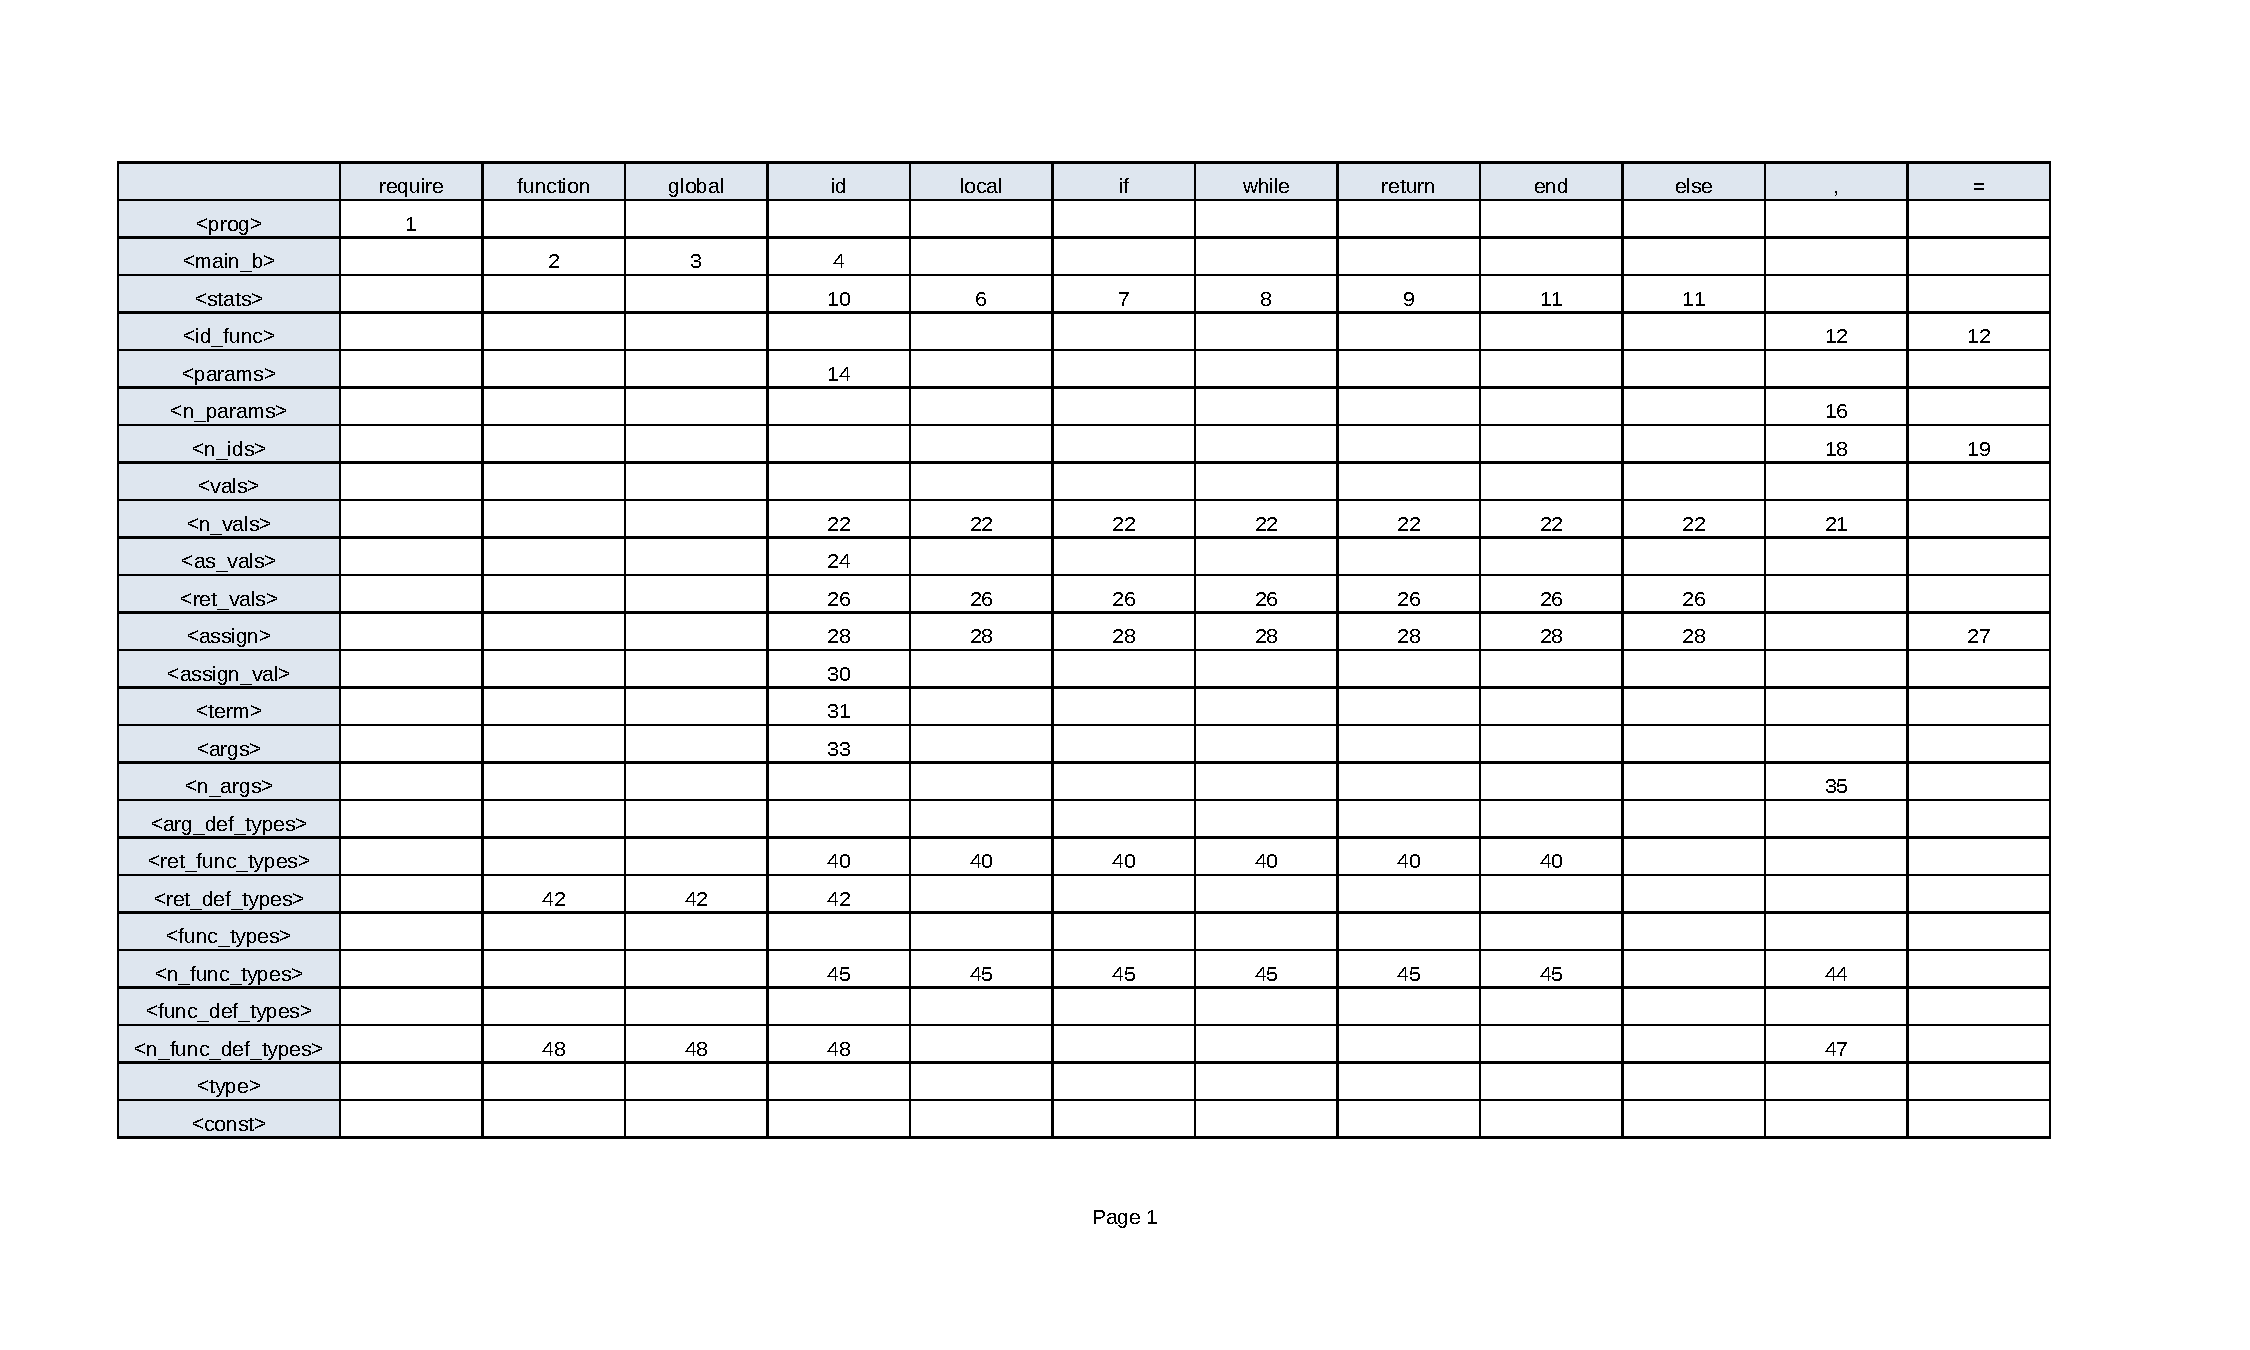
\includegraphics[angle=90,origin=c, width=0.52\textwidth]{images/LL_table_1.pdf}
  \caption{LL tabulka, část 1}
\end{center}
\end{figure}


\newpage

\subsection{Zpracování výrazů}
Precedenční analýza začíná inicializací zásobníku, do kterého je nejprve vložen ukončující terminál. Následně jsou postupně čteny tokeny, přičemž funkce \textit{getOperation()} vyhodnocuje operaci na základě vrcholu zásobníku a aktuálně čteného tokenu. V případě operace \texttt{<} je nad nejvrchnější terminál umístěna zarážka \texttt{<} a čtený token je vložen na vrchol zásobníku. Při operaci \texttt{=} je čtený terminál jednoduše vložen na vrchol zásobníku. Pokud nastane operace \texttt{>}, dochází k pokusu o redukci voláním funkce \textit{tryToMatchRule(t\_Stack *stack)}. Pokud se najde shoda s některým z pravidel gramatiky, probíhá redukce, která zároveň generuje abstraktní syntaktický strom.

Redukce je realizována pomocí funkcí:
\begin{itemize}
    \item \textit{createUnaryExp(t\_Stack *stack)} pro vytvoření unárního výrazu,
    \item \textit{createBinaryExp(t\_Stack *stack)} pro vytvoření binárního výrazu,
    \item \textit{createValueExp(t\_Stack *stack)} pro vytvoření výrazu s hodnotou, nebo id,
    \item \textit{reduceBracketNonTerminal(t\_Stack *stack)} pro redukci v případě (E).
\end{itemize}

Pokud funkce \texttt{getOperation()} vrátí hodnotu \texttt{0}, znamená to chybu, a funkce \texttt{expressionParser(bool tokenRead, ast\_node\_exp\_t **resultPointer)} skončí syntaktickou chybou. V případě, že výsledkem operace je \texttt{1}, provede se kontrola, zda zásobník odpovídá očekávanému stavu \texttt{\$E\$}. Pokud ano, je abstraktní syntaktický strom vložen do ukazatele \texttt{**resultPointer}.


\subsection{Precedenční tabulka}
\begin{figure}[ht!]
\begin{center}
  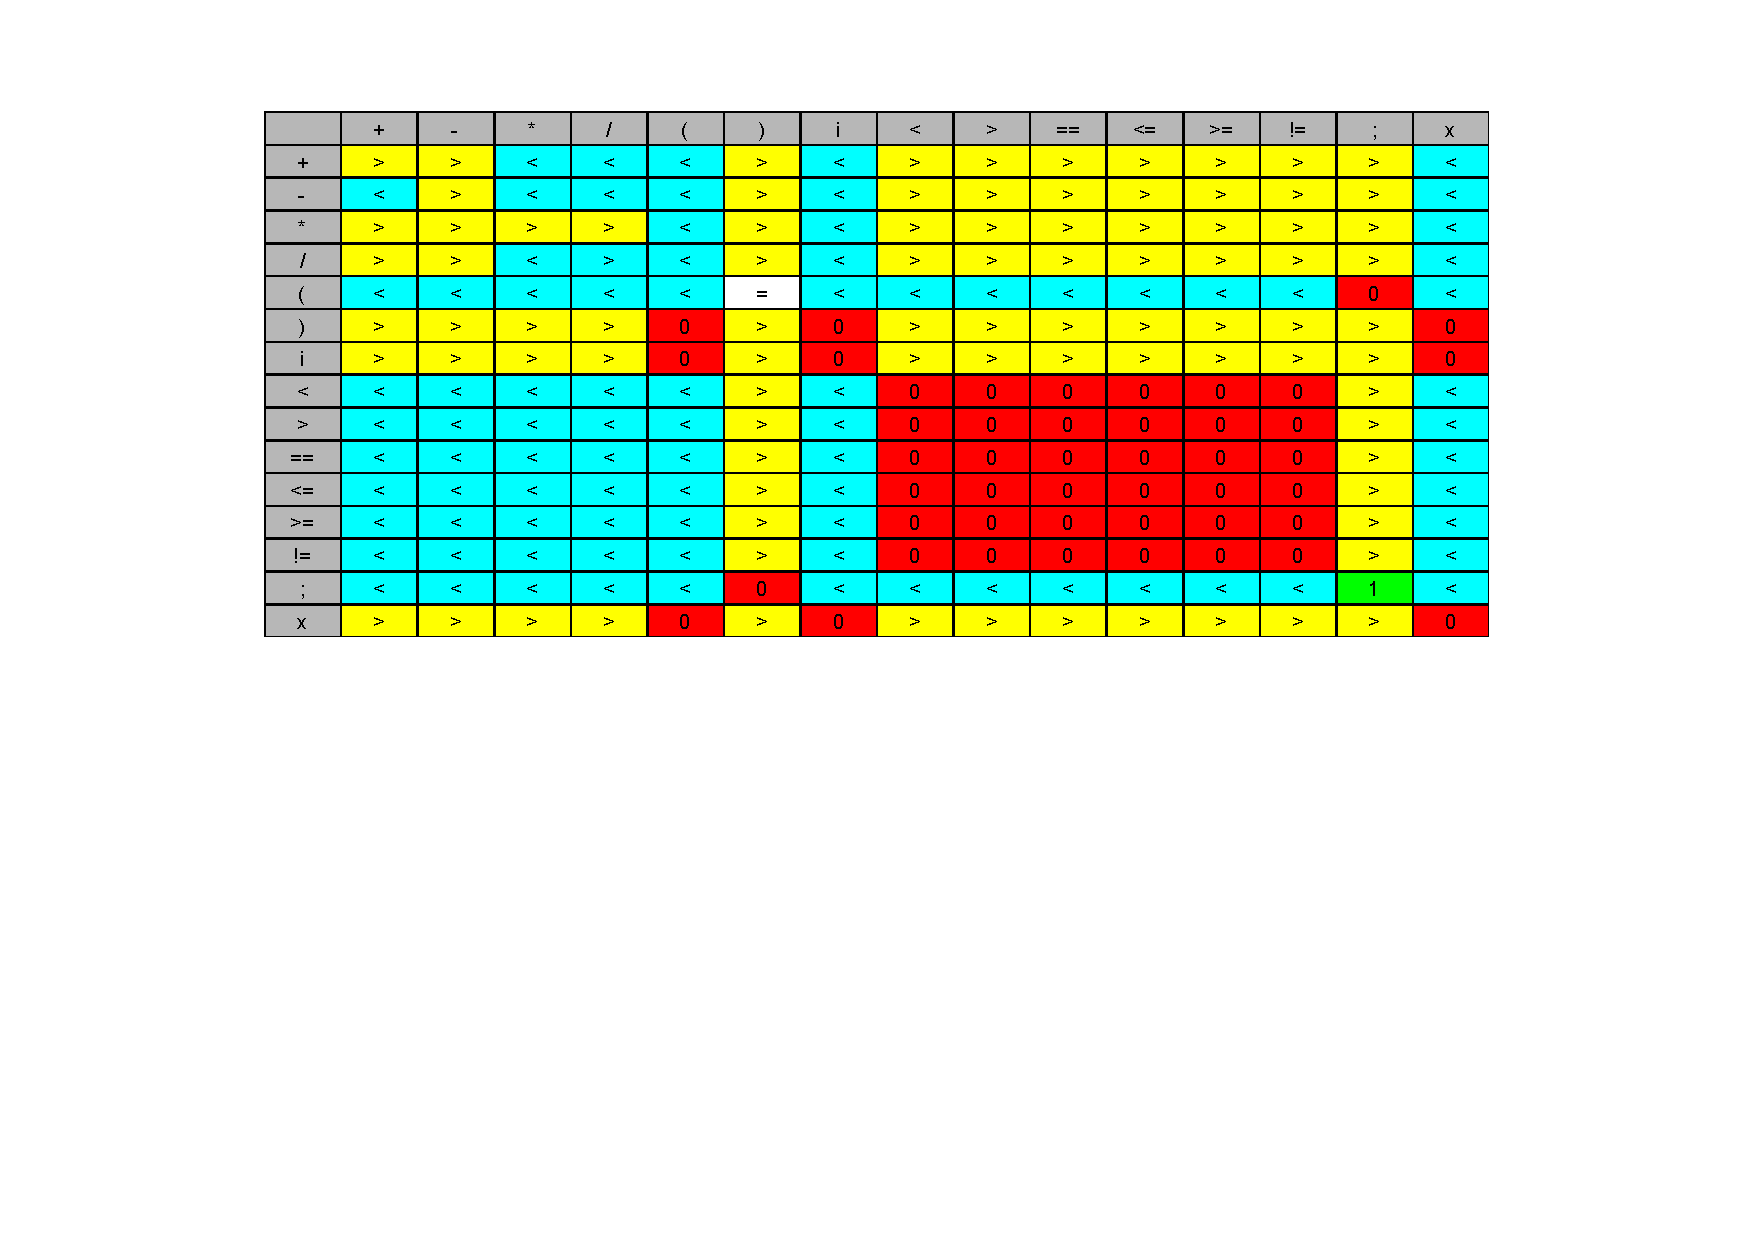
\includegraphics[width=1\textwidth]{images/precedence_table.pdf}
  \caption{Precedenční tabulka}
\end{center}
\end{figure}

\newpage

\subsection{Gramatika pro výrazy}

\begin{enumerate}
    \item $E \to E + E$
    \item $E \to E * E$
    \item $E \to (E)$
    \item $E \to \text{id}$
    \item $E \to \text{num}$
    \item $E \to \text{float}$
    \item $E \to \text{string}$
    \item $E \to E - E$
    \item $E \to E / E$
    \item $E \to E > E$
    \item $E \to E < E$
    \item $E \to E \neq E$
    \item $E \to E \geq E$
    \item $E \to E \leq E$
    \item $E \to E == E$
    \item $E \to -E$
\end{enumerate}

%%%%%%%%%%%%%%%%%%%%%%%%%%%%%%%%%%%%%%%%%%%%%%%%%%%%%%%%%%%%%%%%%%%%%
\newpage
\rhead{\bfseries Implementace překladače (Tabulka symbolů)}
\section{Tabulka symbolů}
Dle výběru varianty zadání TRP-izp je tabulka symbolů implementována tabulkou s rozptýlenými položkami s implicitním zřetězením položek. Ta je implementována v souboru \textit{symtable.c (.h)}. 
\\Na tabulce symbolů jsme začali pracovat dříve než byl zadán druhý projekt z předmětu IAL, a kvůli tomu jsme nemohli využít vzor z něj. Proto jsme rozhodli místo implementace z projektu IAL upravit a použít implementaci tabulky s rozptýlenými položkami z druhého projektu z předmětu IJC.

\subsection{Návrh tabulky symbolů}
Prvek v tabulce symbolů obsahuje následující elementy:

\vspace{1cm}

\begin{itemize}
    \begin{minipage}{0.3\linewidth}   
    \item key
    \item depth
    \item type
    \item returnType
    \item params
    \item paramCound
    \item hasReturn
    \item isConst    
    \item isNullable
    \item isDefined
    \item isUsed
    \item isMutable
    \end{minipage}
    \begin{minipage}{0.65\linewidth}   
    \item[-] název symbolu
    \item[-] hloubka zanoření symbolu
    \item[-] datový typ proměnné
    \item[-] datový typ, který funkce vrací
    \item[-] ukazatel na pole parametrů funkce
    \item[-] počet parametrů
    \item[-] funkce má v těle return    
    \item[-] Symbol je typu const
    \item[-] Symbol může vracet NULL
    \item[-] Symbol byl definován
    \item[-] Symbol byl použit
    \item[-] Symbol může být měněn
    \end{minipage}
\end{itemize}


\newpage

\subsection{Uložení tabulek symbolů do DLL seznamu}
V \textit{symtable.h} je kromě tabulky symbolů definován i seznam \textit{htabs\_l }, který obsahuje odkaz na první a poslední tabulku symbolů. Dvousměrně vázaný lineární seznam je pro odevzdávaný projekt redundantní, ale na začátku projektu jsme počítali s implementací generátoru kódu bez vytváření abstraktního syntaktického stromu, kde byl dvousměrně vázaný seznam vhodnější.\\
\newline
V odevzdávaném projektu existují zároveň nanejvýš dvě tabulky symbolů. První se vytváří na začátku syntaktické analýzy při analýze hlaviček funkcí a ukládají se do ní informace o funkcích. 
\newline
Druhá tabulka se vytváří při vstupu do analýzy funkce a zaniká při ukončení této analýzy.
\vspace{4cm}

\begin{figure}[ht!]
\begin{center}
\begin{tikzpicture}[list/.style={rectangle split, rectangle split parts=2,
    draw, rectangle split horizontal}, >=stealth, start chain]

  \node[list,on chain] (A) {tabulka symbolů funkcí *};
  \node[list,on chain] (B) {tabulka symbolů uvnitř funkce *};
  \node[on chain,draw,inner sep=6pt] (C) {};
  \draw (C.north east) -- (C.south west);
  \draw (C.north west) -- (C.south east);
  \draw[<->] let \p1 = (A.two), \p2 = (A.center) in (\x1,\y2) -- (B);
  \draw[*->] let \p1 = (B.two), \p2 = (B.center) in (\x1,\y2) -- (C);
\end{tikzpicture}


\caption{Diagram dvousměrně vázaného seznamu tabulek symbolů}
\end{center}
\end{figure}
\vspace{4cm}

\rhead{\bfseries Implementace překladače (Sémantická analýza)}
\section{Sémantická analýza}
Sémantická analýza je prováděna zároveň se syntaktickou analýzou v \textit{syntax\_an.c}. Pomocné funkce pro kontrolu sémantiky jsou implementovány v \textit{semantic\_an.c} a definovány v \textit{semantic\_an.h}. Sémantická analýza vrací chybové kódy podle zadání.


%%%%%%%%%%%%%%%%%%%%%%%%%%%%%%%%%%%%%%%%%%%%%%%%%%%%%%%%%%%%%%%%%%%%%%%%%%%%%%%
\newpage
\rhead{\bfseries Generování kódu}
\section{Generování kódu}
Generování kódu funguje na základě průchodu abstraktního syntaktického stromu. Při průchodu se pomocí funkce \textit{printf()} vytváří spustitelný mezikód v instrukční sadě IFJcode24 na standardní výstup. Zdrojový kód pro generování kódu se nachází v souborech \textit{codegen.c} a \textit{codegen.h}. Generátor je tvořen ze dvou částí - tisknutí hlavičky a tisknutí mezikódu na základě vstupu.

\subsection{Tisknutí hlavičky}
Vytisknutí správné hlavičky zajišťuje funkce \textit{printHeaders()}. Tato funkce nejdříve vytiskne povinné záhlaví pro mezikód - \textit{.IFJcode24}. Poté vytiskne skok do funkce main, kterou musí každý vstupní program obsahovat. Následně vytiskne definici jedinné globální proměnné \textit{GF@\_\%} a definice vestavěných funkcí jazyka IFJ24. Definice vestavěných funkcí byly nejdříve napsány a otestovány v pomocném souboru který nebyl odevzdán. Pro názvy proměnných ve vestavěných funkcích je využit znak '\%' na konci, aby nemohlo dojít ke kolizi s proměnnými vytvářenými ve vstupním programu, jelikož znak '\%' není v názvu proměnných povolen.

\subsection{Generování na základě vstupu}
Tato část generování závisí na průchodu abstraktním syntaktickým stromem vytvořeným v předchozích částech. První volanou funkcí je funkce \textit{codebody()}, která prochází tělo(: funkce, while cyklu, if-else) a volá příslušné podpůrné funkce. Jelikož je vstupní program tvořen z funkcí (i main je funkce), začíná se generováním definic funkcí.
\subsubsection{Začátek generování funkcí}
Nejdříve se vytiskne nezměněné jméno funkce pomocí instrukce \textit{LABEL}. Jako první se v každé funkci vytvoří rámec pomocí \textit{CREATEFRAME}, posune se na zásobník pomocí \textit{PUSHFRAME} a následně se nadefinují parametry a návratová hodnota. Poté se zavolá funkce \textit{defAllVars()}, která projde tělo funkce do hloubky(= i do těl cyklů a if-else) a nadefinuje všechny použité proměnné, aby nemohlo dojít ke kolizi kvůli redefinicím. Následně se začne vyhodnocovat samotné tělo uložené v ASS. 
\subsubsection{Generování těla funkce}
Tělo funkce prochází funkce \textit{codebody()}. Pokud narazí na uzel přiřazení, např. \textit{x = 2 + 3}, nejdříve se pravá strana převede do polské notace, tzn. \textit{23+}, a za využití zásobníku je vyhodnocena. Výsledek je následně pomocí instrukce \textit{POPS} uložen do proměnné x. Pokud \textit{codebody()} narazí na uzel volání funkce, vloží se na zásobník argumenty funkce a poté se funkce zavolá pomocí instrukce \textit{CALL}. Pokud \textit{codebody()} narazí na while cyklus nebo if-else vytiskne se \textit{LABEL WHILE\%d}, resp. \textit{LABEL IF\%d}, kde \%d značí číslo určené pomocí globální proměnné \textit{labelCounter}, a to aby bylo možné odlišit vnořené cykly a if-else klauzule. Následně se vytiskne kontrola podmínky a podmíněný skok na \textit{LABEL WHILEEND\%d}, resp. \textit{LABEL ELSE\%d}, pokud nebude podmínka splněna. Následně se zavolá funkce \textit{codebody()} nad tělem while cyklu, resp. if-u. Pokud se jednalo o while cyklus, vytiskne se po tělu cyklu skok na začátek cyklu a \textit{LABEL WHILEEND\%d}. Tímto končí while cyklus. Pokud se jednalo o if, vytiskne se skok za else na \textit{LABEL IFEND\%d} a začátek else \textit{LABEL ELSE\%d}. Pokud se jednalo o if klauzuli i s else částí, zavolá se \textit{codebody()} nad tělem else. Nakonec se vytiskne \textit{LABEL IFEND\%d}. Tímto končí if-else klauzule.
\subsubsection{Konec funkce}
Pokud \textit{codebody()} narazí na return, uloží jeho výsledek do \textit{LF@retval\%}. Na konci funkce se vytiskne instrukce \textit{POPFRAME} a \textit{RETURN}, resp. \textit{EXIT 0} pokud se jednalo o funkci main. Návratová hodnota se následně dá najít jako \textit{TF@retval\%}. Tento proces se provede pro každou funkci ve vstupním zdrojovém kódu.

\section{GNU Make}
Další požadavek projektu bylo vytvoření souboru \textit{Makefile} pro přeložení projektu pomocí příkazu \texttt{make}. Pro kompilaci používáme kompilátor \textit{gcc} s \textit{gnu99} standardem jazyka C. Kompilátor je taky nastavený, aby přerušil překlad při jakékoliv chybě a optimalizace jsou vypnuté.\\
Nástroj GNU Make lze také využít k vytvoření zabaleného archivu pro odevzdání pomocí příkazu \texttt{make zip}.

%%%%%%%%%%%%%%%%%%%%%%%%%%%%%%%%%%%%%%%%%%%%%%%%%%%%%%%%%%%%%%%%%%%%%%%%%%%%%%%%%%%%%
\newpage
\rhead{\bfseries Datové struktury a datové typy}
\section{Datové struktury}

\subsection{Abstraktní syntaktický strom (ASS)}
Abstraktní syntaktický strom, zkráceně ASS, je struktura, kterou vytváříme během syntaktické analýzy a využíváme pro generaci kódu. Jedná se o systém navzájem propojených uzlů. Kořenový uzel je typu \textit{ast\_default\_node} a obsahuje uzly definic funkcí \textit{ast\_node\_fn\_def} a jejich počet. Ty obsahují informaci o funkci s tělo definující funkci. Tělo funkce je pole \textit{ast\_default\_node} ukazujících na uzly níže definované. 
\subsubsection{ast\_node\_fn\_call}
Uzel \textit{ast\_node\_fn\_call} znamená volání funkce. Uchovává informaci o názvu funkce a argumentech s kterými byla volána.
\subsubsection{ast\_node\_fn\_returm}
Uzel \textit{ast\_node\_fn\_return} znamená návrat z funkce. Uchovává informace o návratovém typu a návratové hodnotě uložené v \textit{ast\_node\_exp}.
\subsubsection{ast\_node\_var\_assign}
Uzel \textit{ast\_node\_var\_assign} udává přiřazení do proměnné. Uchovává název proměnné a hodnotu v \textit{ast\_node\_exp}, která se do ní má vložit.
\subsubsection{ast\_node\_var\_def}
Uzel \textit{ast\_node\_var\_def} udává deklaraci proměnné a uchovává název proměnné. Dále pok1ud došlo i k přiřazení do proměnné, uloží jej v \textit{ast\_node\_var\_assign}.\
\subsubsection{ast\_node\_if\_else}
Uzel \textit{ast\_node\_if\_else} udává if-else klauzuli. Uchovává informaci jestli se jedná o if akceptující hodnotu null a tělo a délku těla if i else částí. 
\subsubsection{ast\_node\_while}
Uzel \textit{ast\_node\_while} znamená while cyklus. Uchovává informaci jestli se jedná o if akceptující hodnotu null a tělo a délku těla while cyklu.
\subsubsection{ast\_node\_exp}
Uzel \textit{ast\_node\_exp} ukládá binární strom vytvořený v expression parseru. Navíc má dva speciální ukazatele - v případě volání funkce a v případě znaménka mínus, např. -2.

\subsection{Dynamické pole}
Dynamické pole je použito při generaci kódu pro uchování již definovaných proměnných \textit{array\_vars\_t} a pro řazení exp uzlů v post orderu \textit{array\_items\_t}. Obsahuje pole ukazatelů na ukládané hodnoty, maximální kapacitu a počet momentálně uložených položek.

\subsection{Zásobník}
Zásobník je implementován jako propojený seznam. Obsahuje následující struktury:

\begin{itemize}
    \item \textbf{\texttt{t\_Stack}}: Struktura reprezentující zásobník.
    \begin{itemize}
        \item \texttt{struct StackItem *top} - ukazatel na vrchol zásobníku.
        \item \texttt{int size} - aktuální počet položek v zásobníku.
    \end{itemize}
    \item \textbf{\texttt{t\_StackItem}}: Struktura reprezentující jednu položku v zásobníku.
    \begin{itemize}
        \item \texttt{stackElementType type} - typ položky (\texttt{TERMINAL}, \texttt{NON\_TERMINAL}, \texttt{PRECEDENT\_LESS}).
        \item \texttt{Token *token} - ukazatel na token, který položka obsahuje.
        \item \texttt{struct StackItem *next} - ukazatel na následující položku v zásobníku.
        \item \texttt{struct StackItem *prev} - ukazatel na předchozí položku v zásobníku.
        \item \texttt{ast\_node\_exp\_t *node} - ukazatel na AST uzel asociovaný s touto položkou.
    \end{itemize}
\end{itemize}

Funkce pro práci se zásobníkem:

\begin{itemize}
    \item \textit{void stackInit(t\_Stack *stack)}
    \begin{itemize}
        \item Inicializuje prázdný zásobník.
    \end{itemize}

    \item \textit{int stackPush(t\_Stack *stack, stackElementType type, Token *tkn, ast\_node\_exp\_t *node)}
    \begin{itemize}
        \item Přidá novou položku na vrchol zásobníku.
        \item Vrací \texttt{0} při úspěchu nebo \texttt{INTERNAL\_COMPILER\_ERROR} při chybě alokace paměti.
    \end{itemize}

    \item \textit{void stackPop(t\_Stack *stack)}
    \begin{itemize}
        \item Odstraní položku z vrcholu zásobníku.
    \end{itemize}

    \item \textit{t\_StackItem *stackTop(t\_Stack *stack)}
    \begin{itemize}
        \item Vrací ukazatel na položku na vrcholu zásobníku bez jejího odstranění.
    \end{itemize}

    \item \textit{void stackClear(t\_Stack *stack)}
    \begin{itemize}
        \item Odstraní všechny položky ze zásobníku.
    \end{itemize}

    \item \textit{int stackPushPrecedentLess(t\_Stack *stack)}
    \begin{itemize}
        \item Vloží položku typu \texttt{PRECEDENT\_LESS} za nejbližší \texttt{TERMINAL} položku.
        \item Vrací \texttt{0} při úspěchu, \texttt{INTERNAL\_COMPILER\_ERROR} při chybě alokace paměti nebo \texttt{SYNTACTIC\_ANALYSIS\_ERROR}, pokud \texttt{TERMINAL} neexistuje.
    \end{itemize}

    \item \texttt{t\_StackItem *topTerminal(t\_Stack *stack)}
    \begin{itemize}
        \item Vrací ukazatel na nejbližší položku typu \texttt{TERMINAL} v zásobníku, počínaje od vrcholu.
    \end{itemize}
\end{itemize}

Tento zásobník je klíčovou součástí při implementaci syntaktické precedenční analýzy, kde slouží k ukládání a manipulaci s elementy jako jsou terminály, neterminály a speciální položky pro precedenční analýzu.


%%%%%%%%%%%%%%%%%%%%%%%%%%%%%%%%%%%%%%%%%%%%%%%%%%%%%%%%%%%%%%%%%%%%%%%
\newpage
\rhead{\bfseries Rozšíření a závěr}
\section{Rozšíření}
Naše řešení částečně implementuje rozšíření FUNEXP.\newline
Funkce mohou být volány ve výrazech. Nepodařilo se nám však zavést výrazy jako parametry funkcí, jelikož to syntaktická analýza nepovoluje.

\section{Závěr}
Projekt ze začátku působil velice rozsáhle, ale látku jsme vstřebávali pozvolna a postupně jsme stavěli naše řešení. Znalosti jsme čerpali především z přednášek IFJ a IAL. Nejasnosti ze zadání jsme doplňovali z diskuzního fóra a otázkami na ostatní studenty na Discordu. Jelikož se většina týmu již znala, neměli jsme problém spolupracovat. Správnost řešení jsme ověřovali pokusným odevzdáním a automatickými testy. Projekt jsme stihli vypracovat s jistým předstihem, což nám umožnilo vypracovat tuto dokumentaci. Z projektu jsme si odnesli zkušenosti nejen z programování, ale také z týmové práce a hospodaření s časem.

\end{document}
